
\documentclass[12pt]{article}%
\usepackage{amsmath}%
\usepackage{amsfonts}%
\usepackage{amssymb}%
\usepackage{graphicx}
\usepackage{booktabs}
\usepackage[utf8]{inputenc}
\usepackage{anysize}

\marginsize{2cm}{2cm}{2cm}{2cm} 
\begin{document}

\thispagestyle{empty}

\begin{center}
PONTIFICIA UNIVERSIDAD CATÓLICA DE VALPARAÍSO\\
FACULTAD DE INGENIERÍA\\
ESCUELA DE INGENIERÍA INFORMÁTICA\\

\vspace{4cm}

\Large{\textbf{Diagnosticador de severidad de fallos de rodamientos bajo velocidades variables utilizando la transformada de Fourier y Deep learning}}

\vspace{3cm}

\normalsize{\textbf{Sebastián Ignacio López Norambuena}}\\
\end{center}

\vspace{3cm}
\begin{center} 
Profesor guía: \textbf{Nibaldo Rodríguez Agurto}
\end{center}
\begin{center} 
Profesor co-referente: \textbf{Guillermo Cabrera Guerrero}
\end{center}
\vspace{1cm}
\begin{center} 
Noviembre, 2017
\end{center}
\newpage
\pagenumbering{roman}

\noindent
\Large{\textbf{Resumen}}\\

\normalsize
\noindent El rodamiento es uno de los componentes más utilizados en la maquinaria rotativa. Las fallas en estos elementos son muy comunes y tienen un gran impacto en la cadena de producción de una planta. Por lo tanto, es importante estudiar la tecnología de diagnóstico de fallas en rodamientos e incluirla en los planes de mantenimiento. Una señal de vibración perteneciente a un rodamiento, transporta información dinámica sobre el estado estado de salud de este; así que puede ser utilizada para identificar y clasificar fallas en la estructura de los rodamientos. Para automatizar este proceso, la ingeniería ha propuesto algoritmos de \textit{machine learning} que combinados con técnicas de extracción de características; entregan un diagnóstico óptimo sobre el estado de los rodamientos. Para mejorar el rendimiento de estos modelos cuando la dimensión de los datos de entrada es muy alta, se incluyen técnicas de reducción de dimensionalidad o selección de características. En este documento se propone utilizar esta combinación de técnicas de extracción de características y algoritmos de \textit{deep learning} que reducen la dimensionalidad y realizan un diagnostico de la salud del rodamiento. En la etapa de extracción, se aplicará la transformada rápida de Fourier a una señal de vibración; para obtener la magnitud de los coeficientes y emplearlos como características. Posteriormente una red neuronal profunda compuesta por dos sparse autoencoders y una capa de neuronas con la función de activación softmax, se encargarán diagnosticar la salud del rodamiento.
\newline

\noindent
\textbf{Palabras Clave:} rodamientos, diagnóstico, mantenimiento, señal de vibración, deep learning.

%----------------------Tabla de contenidos-----------------------------%

\newpage
\renewcommand{\contentsname}{Índice}
\tableofcontents
\renewcommand{\figurename}{Figura}
\renewcommand{\refname}{Referencias}
\renewcommand{\listtablename}{Lista de Tablas}
\newpage

%----------------------Tabla de contenidos-----------------------------%

%-------------------------Tabla de imagenes--------------------------%

\renewcommand{\listfigurename}{Lista de Figuras}
\listoffigures
\listoftables
\newpage

%-------------------------Tabla de imagenes--------------------------%

\pagenumbering{arabic}
\section{Introducción}

\paragraph{}
La maquinaria rotativa es ampliamente utilizada en muchos campos industriales y en los últimos años, el monitoreo de condiciones de estas máquinas ha cobrado especial importancia en el mantenimiento moderno. La explicación para esto es que, existe la necesidad de reducir los tiempos de inactividad no programados y los costos asociados al mantenimiento, de manera que se pueda mantener la competitividad corporativa \cite{seeraa}. Con el monitoreo de condiciones se pueden detectar tempranamente fallas potencialmente desastrosas, reduciendo el tiempo de inactividad total de la máquina y de operaciones enteras.

\paragraph{}
Las técnicas de mantenimiento predictivo han demostrado ser estrategias eficaces para reducir fallas inesperadas en la maquinaria. El monitoreo de vibraciones es la tecnología de mantenimiento predictivo más utilizada \cite{zhan}, debido a la cantidad significativa de información que porta la señal sobre el estado salud de la maquinaria. Considerando que los rodamientos son un componente frecuentemente encontrado en la maquinaria rotativa y que pueden causar alrededor del 40-50\% \cite{issam} de todos los desperfectos, muchas investigaciones se centran en el monitoreo de vibraciones para estos componentes.

\paragraph{}
Los rodamientos giran constantemente en condiciones ambientales severas tales como alta temperatura, velocidad de rotación variable y grandes cargas, por lo que presentan una alta frecuencia de rotura \cite{fu}. Realizar un diagnóstico efectivo para los rodamientos es complejo, porque usualmente la señal de vibración tiene un comportamiento no lineal y no estacionario \cite{li}. Este comportamiento de la señal es consecuencia de la compleja estructura mecánica del rodamiento y sus duras condiciones de trabajo.

\paragraph{}
Los sistemas de monitoreo de condiciones son usados para obtener datos en tiempo real de las máquinas. Por lo tanto, enormes colecciones de datos son adquiridas después de un prolongado funcionamiento de estas máquinas. Como los datos generalmente se recopilan más rápido de lo que se tarda en analizarlos, existe la necesidad de un método de diagnóstico que sea capaz de analizar grandes volúmenes de datos y de realizar automáticamente un diagnostico preciso.

\paragraph{}
Este tipo de métodos se denominan \textit{métodos inteligentes de diagnóstico de fallas} y en general, estos están compuestos por dos etapas. La primera etapa consiste en extraer características útiles desde los datos recolectados con alguna herramienta de procesamiento de señales. La segunda etapa utiliza técnicas de inteligencia artificial para distinguir el estado de salud de la maquinaria en base a las características obtenidas en el paso anterior.

\paragraph{}
La primera de estas etapas resulta clave en el diagnóstico de fallas para maquinaria rotativa \cite{guo}, porque reduce la dimensión de los datos, afecta directamente el reconocimiento de patrones y por lo tanto la calidad del diagnóstico. Los métodos convencionales de extracción de características incluyen técnicas en el dominio del tiempo, dominio de la frecuencia y tiempo frecuencia. Diversos autores utilizan estadísticos basados en la forma de la onda en el dominio del tiempo, tales como el valor pico, la media cuadrática, el factor de cresta, el índice de curtosis, la asimetría \cite{zhu}.
 
\paragraph{}
Los principales métodos en el dominio de la frecuencia corresponden a: el cálculo del espectro energético de Fourier \cite{jia}, el espectro de potencia \cite{li} y el análisis cepstral. Respecto a las  técnicas de tiempo frecuencia, suelen ser utilizadas la transformada de Fourier de tiempo corto (STFT), la distribución Wigner-Ville (WVD) y la transformada de paquetes wavelet (WPT). También es posible encontrar otros métodos basados en procesamiento de señales como la descomposición modal empírica (EMD) \cite{yu}, funciones modales intrínsecas (IMF), la transformada wavelet discreta (DWT), la transformada wavelet (WT) \cite{chang} y la transformada Hilbert-Huang (HHT) \cite{rai}.

\paragraph{}
Respecto a las técnicas de inteligencia artificial, aplicadas como clasificador en este contexto, podemos encontrar redes neuronales artificiales (ANN) \cite{ali}, máquinas de vectores de soporte (SVM) \cite{konar}, sistemas Adaptativos de inferencia neuro difusa (ANFIS) \cite{issam}, redes neuronales wavelet (WNN) \cite{wu} y otros. Estas herramientas reciben un entrenamiento con las características obtenidas de la señal de vibración, que ajusta diversos parámetros de sus algoritmos y que hace posible el aprendizaje de patrones ocultos en los datos. Una vez realizado el entrenamiento el clasificador está listo para que, con un nuevo conjunto de atributos de la señal, sea capaz de distinguir si el componente analizado tiene desperfectos o no.

\paragraph{}
De acuerdo a Jia et al. \cite{jia}, los métodos inteligentes de diagnóstico de fallas más comunes emplean ANN's en el segundo paso, dando lugar a dos grandes desventajas. La primera es que la extracción de características depende de la experiencia en procesamiento de señales de los investigadores y se seleccionan según un problema de diagnóstico específico, por lo que probablemente no sean aptas para otros problemas. Y la segunda es que las ANN's utilizadas en estos métodos carecen de arquitecturas profundas, limitando la capacidad de estas para aprender las complejas relaciones no lineales en los problemas de diagnostico de fallas.

\paragraph{}
En función de las investigaciones anteriormente descritas, es que se propone un modelo de diagnóstico de fallas para rodamientos con la transformada de Fourier como técnica de extracción de caracterizaras de la señal, y una red neuronal profunda como clasificador. A diferencia de los instrumentos de clasificación mencionados previamente, la red neuronal profunda utiliza \textit{sparse} autoencoders que reducen la dimensión de las características a la vez que realizan un pre entrenamiento para la capa que realiza la clasificación, lo que mejora el tiempo de entrenamiento y la exactitud de los resultados. Además, se propone la importante adición de las severidades de falla a cada componente del rodamiento, mejorando el nivel de detalle en el que la red neuronal profunda diagnostica las fallas.

\newpage
\section{Definición de objetivos}
\paragraph{}
En esta sección se definen los objetivos general y específicos que persigue la ejecución de este proyecto.
\subsection{Objetivo general}
\paragraph{}
Desarrollar un diagnosticador de severidad de fallos de rodamientos, bajo velocidades variables utilizando la transformada de Fourier discreta.

\subsection{Objetivos específicos}
\paragraph{}
Los objetivos específicos de este proyecto son los siguientes:
\begin{enumerate}
\item{Descomponer señales de vibración con la transformada de Fourier discreta.}
\item{Diseñar e implementar un algoritmo de \textit{deep learning} con sparse autoencoders.}
\item{Evaluar la exactitud del diagnosticador con 4 estados de salud del rodamiento.}
\item{Evaluar la exactitud del diagnosticador con 10 estados de salud del rodamiento.}
\end{enumerate}

\section{Plan de trabajo}
\paragraph{}
Este plan de trabajo utiliza los objetivos específicos como una base, debido a que estos explican las tareas que se deben llevar a cabo para cumplir el objetivo general. Esta segunda entrega, contempla la implementación del modelo propuesto y la evaluación del rendimiento de este. Para la próxima entrega se habrá pulido el marco teórico y la redacción de la investigación en general, sobre todo la discusión de resultados y el estado del arte.

\section{Marco Teórico}

\paragraph{}
Esta sección tiene como objetivo presentar antecedentes, conceptos, definiciones y la importancia de las herramientas y técnicas que se utilizarán en el desarrollo de esta investigación. Comenzando por los antecedentes de la utilización de enfoques en el dominio de la frecuencia, seguido del aprendizaje profundo y finalmente el sustento matemático de ambos.

\paragraph{}
En la literatura especializada existen antecedentes que sirven como base para esta investigación, un ejemplo de estos es \cite{mao}, donde se utiliza la transformada de Fourier para extraer características de una señal y usar la energía contenida en el espectro de frecuencias como entrada a 3 clasificadores: una red neuronal artificial, autoencoders apilados y una red con \textit{extreme learning machine}. Este ejemplo corresponde a un excelente antecedente debido a que implementa la misma técnica de extracción de características y clasificador que este trabajo, con la salvedad que sus autoencoders no incluyen la dispersión de los nodos en la capa oculta, variación denominada \textit{sparse} autoencoder y que si se usa en esta investigación.

\paragraph{}
Otro ejemplo de un antecedente es \cite{kanpaj} en donde se postula que el análisis espectral o dominio de la frecuencia, es el enfoque más utilizado para detectar fallas en los rodamientos. Dado que los enfoques en el dominio del tiempo solo pueden detectar cuándo ocurre una falla en el rodamiento, mientras que el análisis espectral además puede determinar en qué componente del rodamiento se encuentra el desperfecto. También se explica que la transformada rápida de Fourier es el algoritmo computacionalmente eficiente para convertir una señal en el dominio del tiempo a componentes de frecuencia discretos.

\paragraph{}
En cuanto a los antecedentes de redes neuronales profundas podemos encontrar a \cite{ran}, donde proponen la utilización de una red neuronal profunda sin autoencoders para diagnosticar una señal de vibración de un rodamiento. Los autores no utilizan métodos de extracción de características, y solo dividen en segmentos la señal original para entregársela a la red neuronal profunda. El argumento de los autores es que se debe mantener la coherencia temporal de la señal, pero la cantidad de datos que recibe la red es enorme, resultando en grandes tiempos de entrenamiento y una gran capacidad de cómputo.

\paragraph{}
A continuación se encuentran los conceptos y definiciones matemáticas de las herramientas que se utilizarán en esta investigación, comenzando por la transformada de Fourier y sus variantes, seguido del \textit{deep learning} (o aprendizaje profundo), los autoencoders y su variante \textit{sparse} autoencoder.

\subsection{Transformada de Fourier}
\paragraph{}
La transformada de Fourier es una herramienta matemática poderosa, por lo que es utilizada en diversos campos de la ciencia y la ingeniería. Puede ser vista como la transformación de una señal en un dominio (típicamente tiempo o espacio) a otro dominio, el dominio de la frecuencia. Al aplicar la transformada de Fourier a una señal, se obtienen sus componentes fundamentales en frecuencia que a menudo revelan estructuras ocultas, que en el dominio del tiempo, no son posibles de observar.

\paragraph{}
Como consecuencia de lo anterior, el análisis de Fourier está en la base de muchas teorías de la ciencia y juega un papel fundamental en el diseño práctico de la ingeniería. El alcance actual de la influencia del análisis de Fourier está indicado por una lista parcial de científicos e ingenieros que la utilizan \cite{robert}:

\begin{itemize}
\item{Los ingenieros de audio utilizan técnicas de Fourier, en parte porque el oído parece ser sensible al comportamiento del dominio de frecuencia.}
\item{Los estadísticos y probabilistas caracterizan y calculan las distribuciones de probabilidad usando transformadas de Fourier. Las transformadas de Fourier de las funciones de covarianza se utilizan para caracterizar y estimar las propiedades de los procesos aleatorios.}
\item{Los radioastrónomos utilizan la transformada de Fourier para formar imágenes a partir de datos interferométricos recogidos por arreglos de antenas.}
\item{Los cristalógrafos encuentran las estructuras cristalinas usando transformadas de Fourier de los patrones de difracción de rayos X.}
\item{Los ingenieros biomédicos recogen datos en el dominio de la frecuencia y luego los transforman
inversamente con Fourier para obtener imágenes de resonancia magnética.}
\end{itemize}

\subsubsection{Transformada de Fourier continua}
\paragraph{}
La transformada de Fourier continua es resultado de la generalización de las series de Fourier. Puede aplicarse prácticamente a cualquier función, no requiere que la función sea periódica, y para datos discretos, puede ser evaluada rápidamente usando una técnica moderna llamada transformada de Fourier Rápida (FFT). La transformada de Fourier de una función $f(t)$ se define \cite{anthony} como:

\begin{equation}
F(\omega)=\int_{-\infty}^{\infty}f(t)e^{-i{\omega}t}dt
\end{equation}

\paragraph{}
Donde $\omega$ es igual a la frecuencia angular $2{\pi}f$, y $F(\omega)$ es una función continua de valores complejos. Una vez que se ha determinado una transformada de Fourier, la función original $f(t)$ puede ser recuperada a partir de la transformada de Fourier inversa:

\begin{equation}
f(t)=\frac{1}{2\pi}\int_{-\infty}^{\infty}F(\omega)e^{i{\omega}t}d\omega
\end{equation}

\subsubsection{Transformada de Fourier discreta}

\paragraph{}
La transformada discreta de Fourier (DFT) (Ecc. \ref{dft}), como lo indica su nombre, opera sobre un número finito de datos y es discreta en ambos dominios, el del tiempo y el de la frecuencia. La DFT trabaja sobre un bloque de $N$ muestras de la secuencia $x(n)$ y entrega $N$ componentes de frecuencia indexadas mediante la variable entera $k$.

\begin{equation}
\label{dft}
X(k) = \sum_{n=0}^{N-1}x(n)e^{-j(2\pi/N)kn} \quad , 0 \leq k \leq N-1
\end{equation}

\paragraph{}
La transformadas discreta de Fourier inversa, o IDFT está dada por la Ecc. \ref{idft}, la cual recibe $N$ componentes de frecuencia y entrega $N$ muestras de la secuencia $x(n)$. La fórmula es muy similar a la de la DFT, se distingue en el signo del exponente de $e$ y en la presencia del factor de normalización $1/N$. Ambas diferencias son necesarias para que se cumpla la condición de la Ecc. \ref{condition}.

\begin{equation}
\label{idft}
x(n)=\frac{1}{N}\sum_{k=0}^{N-1}X(k)e^{j(2\pi/N)kn} \quad ,0 \leq n \leq N-1
\end{equation}

\begin{equation}
\label{condition}
x(n) = IDFT[DFT[x(n)]]
\end{equation}

\subsubsection{Transformada de Fourier de tiempo corto}
\paragraph{}
Consideremos una señal $x(t)$ y supongamos que es estacionaria cuando se ve a través de una ventana $w(t)$, cuya duración es $T$, centrada en la posición de tiempo $\tau$, la transformada de Fourier de la señal en ventana $x(t)$ es la transformada de Fourier de corto tiempo \cite{yufeng} (STFT):

\begin{equation}
\label{stft}
X(\tau,\omega)=\int_{-\infty}^{\infty}x(t)w(t-\tau)e^{-j\omega{t}}dt
\end{equation}

\paragraph{}
Esta transformada mapea la señal desde el dominio del tiempo en un plano de tiempo-frecuencia conjunto $(\tau,f)$. Para la implementación, la versión discreta de la Ecc. \ref{stft} debe utilizarse como:

\begin{equation}
X_{n}(e^{jw_{k}})=\sum_{m=-\infty}^{\infty}w(n-m)x(m)e^{-jw_{k}m}
\end{equation}

\paragraph{}
Donde $n$ y $k$ $(1{\leq}k{\leq}N)$ son el tiempo discreto y la frecuencia respectivamente, y $N$ es la longitud de la ventana

\subsection{Deep learning}
\paragraph{}

En los años recientes un nuevo enfoque de \textit{machine learning} denominado \textit{deep learning}, ha llamado la atención de investigadores de múltiples áreas debido a una serie de ventajas respecto a otros enfoques. El \textit{deep learning} ha tenido un gran impacto en trabajos actuales de reconocimiento de voz, visión artificial y procesamiento del lenguaje natural, debido a la efectividad empírica de este respecto a enfoques alternativos en este ámbito. El desarrollo de esta tecnología fue potenciado en gran medida por la creciente capacidad de cómputo de los equipos, y por el uso de los inmensos volúmenes de datos que son generados todos los días por la humanidad.

\paragraph{}
Esta ola de interés por el \textit{deep learning}, se centra principalmente en los perceptrón multicapa profundo (deep multilayer perceptron), las redes convolucionales profundas (deep convolutional network) y las redes neuronales recurrentes (recurrent neuronal network) de acuerdo a Witten (2016) \cite{mining}. Sin embargo, la mayoría de los métodos de \textit{deep learning} se basan en el perceptrón multicapa profundo, porque lo utilizan como el bloque esencial de construcción. El \textit{deep learning} formula el problema subyacente como una arquitectura en forma de red, en la que su capa de salida define una función de costos (también llamada función de perdida) que es necesaria para aprender.

\paragraph{}
El desarrollo del \textit{deep learning} está relacionado con el uso de técnicas de aprendizaje no supervisado como los diferentes tipos de autoencoder que existen para realizar un pre entrenamiento de las capas ocultas. Y es que uno de los principales propósitos del aprendizaje no supervisado es producir buenas representaciones de los datos \cite{ranzato} que puedan ser usadas para la detección, reconocimiento, predicción o visualización. Las buenas representaciones eliminan variaciones irrelevantes de los datos de entrada, mientras que se preserva la información que es útil para la tarea a realizar.

\paragraph{}
El aprendizaje no supervisado tiene la habilidad de crear jerarquías de características profundas (deep features hierarchies) mediante el apilado de módulos no supervisados uno encima de otro, habilidad que es frecuentemente utilizada en el \textit{deep learning}. Un módulo no supervisado de un nivel en la jerarquía se alimenta con los vectores de representación producidos por el nivel inferior. Las representaciones de nivel superior captan las dependencias de alto nivel entre las variables de entrada, mejorando así la capacidad del sistema para capturar las regularidades subyacentes en los datos.

\subsubsection{Autoencoders}
\paragraph{}
Un autoencoder (AE) es una red neuronal artificial no supervisada de tres capas que es entrenada para replicar los datos de entrada en la salida. El entrenamiento de los autoencoder es no supervisado en el sentido de que no requiere datos etiquetados para aprender a replicarlos en la salida. Este tipo especial de red neuronal es utilizada para pre entrenar las capas ocultas de las redes neuronales profundas, de manera que encuentran pesos sinápticos que agilizan la búsqueda de mínimos globales para la función de costos. Los AE mejoran la capacidad de generalización en la tarea de clasificar y reducen la dimensión de los datos de entrada a medida que se transforman en las capas ocultas.

\begin{figure}[ht]
  \centering
    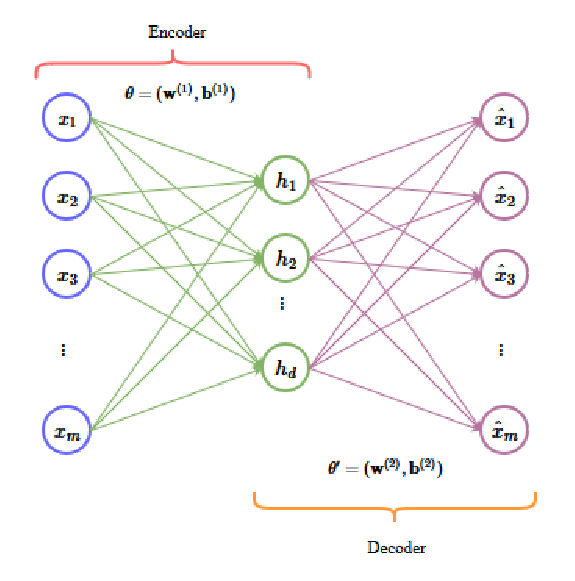
\includegraphics{./AE.eps}
  \caption{Diagrama que ilustra la estructura de un autoencoder formado por la red encoder (lado izquierdo) y la red decoder (lado derecho) con sus respectivos parámetros de entrenamiento.}
  \label{fig:ae}
\end{figure}

\paragraph{}
Es posible identificar dos estructuras en la red autoencoder, por una parte el codificador en el lado izquierdo de la Fig. \ref{fig:ae}, que mapea los datos de entrada desde un espacio de alta dimensión en códigos de un espacio de baja dimensión. Por otra parte, que se encuentra al lado derecho de la Fig. \ref{fig:ae}, reconstruye los datos de entrada a partir de los códigos obtenidos por la capa oculta llevándolos a su dimensión original \cite{shao}. Ahora que está claro cuál es el encoder y el decoder, podemos definir matemáticamente ambas estructuras.

\paragraph{}
Dadas las muestras de entrenamiento $\textbf{x}=(x_{1},x_{2},...,x_{n})$, donde la muestra $x_{n}\in \mathbb{R}^{m}$, se define la red encoder como una función codificadora $f_{\theta}$ (Ecc. \ref{f}) cuya tarea es representar estas muestras en un vector con códigos de menor dimensión denominado $\textbf{h}=(h_{1},h_{2},...,h_{n})$, en donde $h_{n} \in \mathbb{R}^{d}$ y $d<m$. La matriz de pesos sinápticos de la función encoder corresponde a $\textbf{w}^{(1)} = (w_{1}^{(1)},w_{2}^{(1)},...,w_{m}^{(1)})$ con $w_{m}^{(1)}\in \mathbb{R}^{d}$, mientras que $\textbf{b}^{(1)}=(b_{1}^{(1)},b_{2}^{(1)},...,b_{d}^{(1)})^T$ representa el arreglo de \textit{biases} pertenecientes a las neuronas de la capa oculta. Los pesos sinápticos y los \textit{biases} conforman $\theta$, el conjunto de parámetros a minimizar en la función de costos que será detallada más adelante.

\begin{equation}
\label{h}
\textbf{h}=f_{\theta}(\textbf{x})
\end{equation}

\begin{equation}
\label{f}
f_{\theta}(\textbf{x})=s_{f}(\textbf{w}^{(1)}\textbf{x}+\textbf{b}^{(1)})
\end{equation}

\begin{equation}
\label{teta1}
\theta=(\textbf{w}^{(1)},\textbf{b}^{(1)})
\end{equation}

\paragraph{}
La red decoder se define como una función de reconstrucción denotada como $g_{\theta'}$ (Ecc. \ref{g}), dicha función mapea el vector $\textbf{h}$ desde el espacio de baja dimensión en el que se encuentra, de vuelta al espacio de alta dimensión original realizando así la reconstrucción. Los datos reconstruidos se denotan mediante $\hat{\textbf{x}}=(\hat{x}_{1},\hat{x}_{2},...,\hat{x}_{n})$ (Ecc. \ref{xhat}), en donde $\hat{x}_{n}\in \mathbb{R}^{m}$. El primer parámetro que compone a $\theta'$ perteneciente al decoder, es la matriz de pesos sinápticos de salida $\textbf{w}^{(2)} = (w_{1}^{(2)},w_{2}^{(2)},...,w_{m}^{(2)})$ con $w_{m}^{(2)}\in \mathbb{R}^{d}$. Mientras que el segundo, es el arreglo de \textit{biases} $\textbf{b}^{(2)}=(b_{1}^{(2)},b_{2}^{(2)},...,b_{d}^{(2)})^T$. 
\begin{equation}
\label{xhat}
\hat{\textbf{x}}=g_{\theta'}(\textbf{h})
\end{equation}

\begin{equation}
\label{g}
g_{\theta'}(\textbf{h})=s_{g}(\textbf{w}^{(2)}\textbf{h}+\textbf{b}^{(2)})
\end{equation}

\begin{equation}
\label{teta2}
\theta'=(\textbf{w}^{(2)},\textbf{b}^{(2)})
\end{equation}

\paragraph{}
Los conjuntos de parámetros $\theta$ y $\theta'$ de las redes encoder y decoder respectivamente, son aprendidos simultáneamente en la tarea de reconstruir en la mayor medida posible los datos originales de entrada. En otras palabras, es deseable obtener el menor error de reconstrucción (Ecc. \ref{xi}) posible a través de las $n$ muestras de entrenamiento, utilizando el error cuadrático medio (MSE). Este estimador es la función de costo estándar para los autoencoder y muchos otros algoritmos de \textit{machine learning} \cite{mining}.

\begin{equation}
\label{xi}
J_{mse}(\theta,\theta')=\frac{1}{2n}\sum_{i=1}^{n}{\|x_{i}-\hat{x}_{i}\|}^2
\end{equation}

\paragraph{}
El proceso de aprendizaje del autoencoder puede ser visto como un problema de optimización porque tiene como objetivo encontrar los conjuntos de parámetros $\theta$ y $\theta'$ que minimizan el error de reconstrucción. La función de costos que debemos optimizar (Ecc. \ref{fcost}), también llamada función de pérdida, se compone por el error de reconstrucción (Ecc. \ref{xi}) y otro término llamado \textit{weight decay} (Ecc. \ref{weight}), que penaliza los pesos de entrada y salida para evitar el sobre entrenamiento u \textit{overfitting}.

\begin{equation}
\label{weight}
J_{weight}(\theta,\theta')=\frac{\lambda}{2}\sum_{l=1}^{2}\sum_{i=1}^{s_l}\sum_{j=1}^{s_{l+1}}({w^{(l)}_{ji}})^2 \quad s_{1}=m,s_{2}=d,s_{3}=m.
\end{equation}

\paragraph{}
El término \textit{weight decay} de acuerdo a \cite{haykin}, fuerza a algunos de los pesos sinápticos a tomar valores cercanos a 0, mientras que permite a otros pesos a mantener sus relativos grandes valores. Algunos pesos sinapticos tienen muy poca influencia en el desempeño de la red neuronal y debido a que tienen una pobre capacidad de generalización, provocan que la red se sobre entrene. En la Ecc. \ref{weight}, $\beta$ comúnmente parámetro de ajuste de pesos, es el encargado de penalizar a los pesos sinápticos.

\begin{equation}
\label{fcost}
\phi_{AE}(\theta,\theta')= J_{mse}(\theta,\theta') + J_{weight}(\theta,\theta')
\end{equation} 

\paragraph{}
Ahora que hemos definido la función de costo (Ecc. \ref{fcost}) de los autoencoder estándar, generalmente se utiliza el algoritmo \textit{backpropagation} como en muchas otras técnicas de \textit{machine learning} con el fin de actualizar sus pesos sinápticos y \textit{biases} y así disminuir en la mayor medida posible el error de reconstrucción. Este algoritmo calcula el gradiente a la función de costos para encontrar direcciones que permiten actualizar los pesos y \textit{biases} iniciales, de manera que con cada iteración se acerquen más al mínimo global de la función. Una vez hallados los parámetro óptimos, la capa oculta $\textbf{h}$ del autoencoder es capaz de representar a los datos de entrada en una dimensión menor que la original sin perder información relevante para el reconocimiento de patrones.

\subsubsection{Sparse autoencoders}

\paragraph{}
Podemos definir al \textit{sparse} autoencoder, desde ahora denominado SAE, como una extensión del autoencoder estándar, que obliga a sus unidades de la capa oculta a mantener una baja activación media. Creando así características dispersas que logran una mejor generalización por parte del clasificador \cite{du}. El \textit{sparse} autoencoder impone un término de penalización a las unidades de la capa oculta, forzando a que la activación media de cada unidad sea cercana al parámetro de dispersión $\rho$ que generalmente toma un valor muy pequeño cercano a 0. 

\begin{equation}
\label{sparse}
\phi_{SAE}(\theta,\theta')=\phi_{AE}(\theta,\theta')+J_{sparse}(\theta,\theta')
\end{equation}

La restricción se hace efectiva agregando el término de penalización a la función de costos del autoencoder estándar $\phi_{AE}$ (Ecc. \ref{fcost}), resultando en una nueva función de costos $\phi_{SAE}$ (Ecc. \ref{sparse}).

\begin{equation}
J_{sparse}(\theta,\theta')=\beta\sum_{j=1}^{d}KL(\rho||\hat{\rho_{j}})
\end{equation} 

\begin{equation}
\label{kl}
KL(\rho||\hat{\rho_{j}})={\rho} \log\frac{\rho}{\hat{\rho_{j}}}+(1-\rho)\log\frac{1-\rho}{1-\hat{\rho_{j}}}
\end{equation} 

\begin{equation}
\label{rho}
\hat{\rho_{j}}=\frac{1}{n}\sum_{k=1}^{n}h_{j,k}
\end{equation} 

\paragraph{}
$J_{sparse}$ corresponde al término incorporado que impone la restricción de dispersión, en donde $\beta$ controla el peso de este nuevo término y $KL(\rho||\hat{\rho_{j}})$ (Ecc. \ref{kl}) es la divergencia Kullback-Leibler entre una variable aleatoria Bernoulli con media $\rho$ y una variable aleatoria Bernouilli media $\hat{\rho_{j}}$. La divergencia KL es una función estándar para medir la diferencia entre dos distribuciones de probabilidad diferentes. 
Definiremos $\hat{\rho_{j}}$ (Ecc. \ref{rho}) como la probabilidad media de activación en la j-ésima unidad de la capa oculta $\textbf{h}$ a través las $n$ muestras, y $\rho$ la probabilidad de activación deseada ($\rho\ll1$) \cite{song}. 

\paragraph{}
Una vez que hemos definido el término de dispersión y lo hemos incorporado a la función de costos del autoencoder (Ecc. \ref{scost}), aplicaremos el método del gradiente conjugado para actualizar los pesos y \textit{biases}. El método del gradiente conjugado pertenece a una clase de métodos de optimización de segundo orden conocidos colectivamente como métodos de dirección conjugada \cite{haykin}. La motivación para utilizar este método es que converge mas rápido hacia un mínimo que el descenso del gradiente, y a la vez se evitan los requisitos de computación y almacenamiento del hessiano, como lo requiere el método de Newton.

\begin{equation}
\label{scost}
\phi_{SAE}(\theta,\theta')=\frac{1}{2n}\sum_{i=1}^{n}{\|x_{i}-\hat{x}_{i}\|}^2 + \frac{\lambda}{2}\sum_{l=1}^{2}\sum_{i=1}^{s_l}\sum_{j=1}^{s_{l+1}}({w^{(l)}_{ji}})^2 + \beta\sum_{j=1}^{d}KL(\rho||\hat{\rho_{j}})
\end{equation} 

Para simplificar la notación del método, definiremos $\Theta$ (Ecc. \ref{param}) como un arreglo que contiene los parámetros de la función de costos. Según la Ecc. \ref{gconjugado}, este método toma los parámetros iniciales y los actualiza sumándoles una dirección multiplicada por una tasa de aprendizaje denominada $\eta$. El arreglo que contiene las direcciones (Ecc. \ref{direcciones}) se obtiene utilizando la dirección previa multiplicada por el parámetro conjugado $\gamma$ más el residuo (Ecc. \ref{residuo}). El arreglo gradiente (Ecc. \ref{gradiente}) está compuesto por las derivadas parciales de la función de costos, a la vez que la derivada parcial $\frac{\partial{\phi_{SAE}}}{\partial{\theta}}$ se compone de las derivadas parciales de pesos y \textit{biases} (Ecc. \ref{parcial}).

\begin{equation}
\label{param}
\Theta = (\theta,\theta')
\end{equation} 

\begin{equation}
\label{gconjugado}
\Theta(n+1)=\Theta(n)+{\eta}s(n)
\end{equation}

\begin{equation}
\label{direcciones}
s(n+1)=r(n+1)+\gamma{s(n)}
\end{equation} 

\begin{equation}
\label{residuo}
r(n+1) = -\nabla{\phi_{SAE}(\Theta(n+1))}
\end{equation} 

\begin{equation}
\label{gradiente}
\nabla{\phi_{SAE}} = \left(\frac{\partial{\phi_{SAE}}}{\partial{\theta}},\frac{\partial{\phi_{SAE}}}{\partial{\theta'}}\right)
\end{equation}

\begin{equation}
\label{parcial}
\frac{\partial{\phi_{SAE}}}{\partial{\theta}} = \left(\frac{\partial{\phi_{SAE}}}{\partial{\textbf{w}^{(1)}}},\frac{\partial{\phi_{SAE}}}{\partial{\textbf{b}^{(1)}}}\right)
\end{equation}  
\subsection{Método de diagnóstico basado en DNN}
\label{sec:training}

\paragraph{}
En esta sección se dará detalle al proceso de entrenamiento de la red neuronal profunda (DNN) y los elementos que la componen. La red utilizada en este modelo, posee una capa de entrada, dos capas ocultas y una capa de salida con la función de transferencia softmax. Las dos capas ocultas son pre entrenadas con dos \textit{sparse} autoencoder (SAE) respectivamente. Estas redes de tres capas permiten encontrar los parámetros de entrenamiento a la vez que reducen la dimensión de los datos de entrada codificandolos en un espacio de menor dimensión. 

\paragraph{}
Una vez que el primer SAE termina de aprender su representación de los datos a través del algoritmo del gradiente conjugado (Ecc. \ref{gradiente}), inicializa con sus parámetros óptimos $\theta_{1}$ a la primera capa oculta de la DNN como se muestra en la parte izquierda A de la Fig. \ref{fig:deepnet}. Luego el segundo SAE, constituido por la primera y la segunda capa oculta de la DNN, aprende un conjunto de parámetros que inicializa a la segunda capa oculta y los códigos de la segunda capa oculta alimentan a la regresión softmax para que sea entrenada.

\paragraph{}
Una vez obtenidos los parámetros de las capas ocultas, la DNN realiza un \textit{fine tuning} que básicamente es aplicar el algoritmo \textit{backpropagation} a la red entera para mejorar los pesos y \textit{biases} en conjunto. Se utiliza el descenso del gradiente en vez del gradiente conjugado porque los parámetros se encuentran cerca del mínimo global de la función de costos, por lo que no son necesarias demasiadas iteraciones en el proceso.


\begin{figure}[ht]
  \centering
    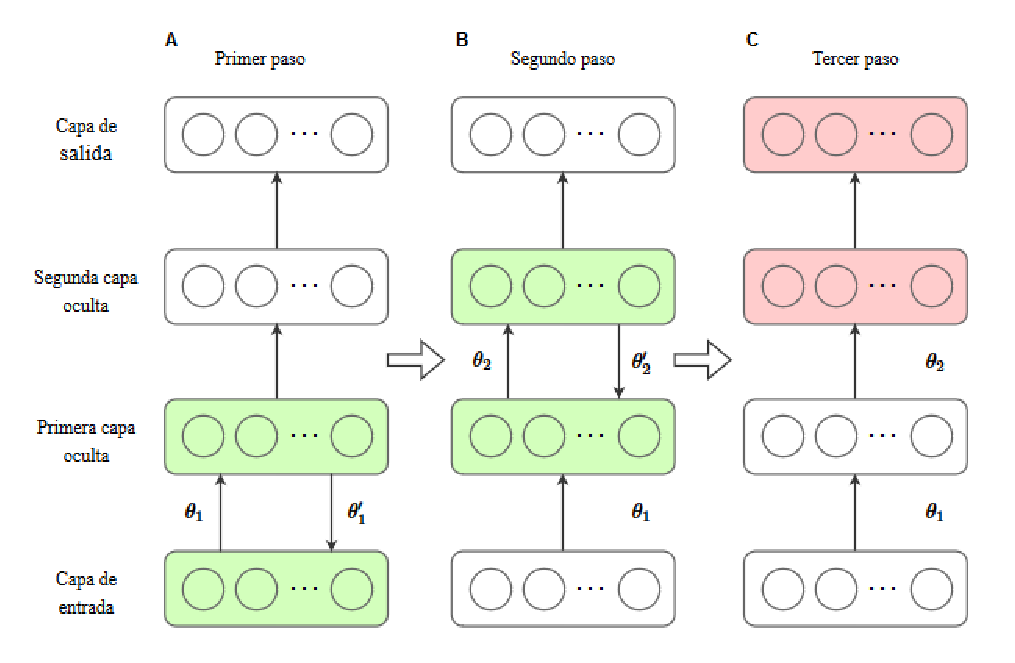
\includegraphics[scale=0.9]{./training.eps}
  \caption{Diagrama que representa el entrenamiento de los \textit{sparse} autoencoder y la asignación de sus parámetros a la DNN}
  \label{fig:deepnet}
\end{figure}

\section{Experimento y resultados}
\label{sec:exp}

\subsection{Datos experimentales}
\label{sec:datos}
\paragraph{}
Los datos utilizados en este trabajo corresponden a señales de vibración de un rodamiento de bolas, obtenidos de un experimento realizado por el Bearing Data Center of Case Western Reserve University \cite{case}. Los aparatos empleados en este laboratorio de vibraciones corresponden a: un motor de 2 hp a la izquierda del banco de pruebas (como se aprecia en la Figura \ref{fig:bearing}), un transductor/codificador de torque en el centro y un dinamómetro a la derecha. Un acelerómetro es el encargado de registrar las señales de vibración emitidas por el rodamiento que soporta el eje del motor.

\begin{figure}[ht]
  \centering
    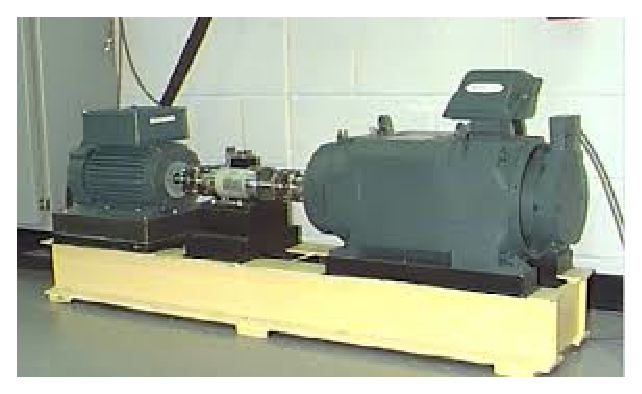
\includegraphics[scale=0.8]{./bearing.eps}
  \caption{Ilustración del experimento realizado por la Case Western Reserve University \cite{case}}
  \label{fig:bearing}
\end{figure}

\paragraph{}
El rodamiento ubicado en el \textit{drive end} fue sometido a descargas eléctricas que generaron defectos en un sólo punto, con tres diámetros de falla: 0.007, 0.014 y 0.021 pulgadas. Estos defectos son inducidos bajo velocidades de rotación variables de 1730, 1750 1772 y 1792 RPM y 4 diferentes cargas de 0, 1, 2 y 3 caballos de fuerza respectivamente. Por lo que los datos pueden ser organizados en conjuntos de datos separados por velocidad/carga como se detallará en la siguiente sección. La frecuencia de muestreo es de 12 kHz para las cuatro condiciones de salud: normal (N), falla en el anillo externo (OF), falla en el anillo interno (IF) y falla en la bola (RF). 

\paragraph{}
El motivo para utilizar esta base de datos es que sirve como punto de comparación con investigaciones que realizan diagnóstico de fallas a rodamientos. Permitiendo sacar conclusiones acerca de los tiempos de entrenamiento, desempeño del diagnóstico y ventajas y desventajas del modelo propuesto. Además, al tener tipos de fallas con severidades, es posible diagnosticar un problema de mayor complejidad y llevar al límite la capacidad de diagnóstico del modelo.

\subsection{Construcción de los datasets}
\label{sec:datasets}

\paragraph{}
Con el objetivo de probar la capacidad de diagnósticos del modelo, se utilizarán 5 conjuntos de datos separados por velocidad/carga, tipo de falla y severidad. En su interior hay 10 carpetas con las señales de vibración, por ejemplo: para el tipo de falla anillo interno habrá 3 carpetas con las señales de vibración de las tres severidades de la falla. El \textit{dataset} E, es especial debido a que tiene las 4 velocidades juntas, por lo que en las 10 carpetas se encuentran las señales de vibración por tipo de falla y severidad para las 4 velocidades; resultando en el \textit{dataset} más grande y complejo de diagnosticar.

\paragraph{}
Las señales utilizadas para construir los conjuntos de datos corresponden a las que fueron medidas en el \textit{drive end} (DE) del sistema Fig. \ref{fig:bearing}. La principal razón para utilizar estas señales es que el acelerómetro con el que se tomaron las muestras se encontraba cerca del rodamiento observado, por lo que las señales son menos afectadas por la atenuación y el ruido. En la Tabla \ref{table:tdatasets} se aprecia cada uno de los 5 conjuntos de datos, con 58 muestras por señal consecuencia de un tamaño de segmentación igual a 2048 obtenido de un largo proceso de \textit{tunning}.

\paragraph{}
Como se explicaba en párrafos anteriores, el \textit{dataset} E es el más grande porque reúne las 5 cargas y es que mas nos interesa de las pruebas porque los rodamientos en un sistema real trabajan bajo velocidades y cargas variables. Lo que implica que la señal de vibración resultante es no lineal y no estacionaria, de manera que el diagnóstico de fallas se torna complejo como se explicaba en la introducción de este trabajo. Otro \textit{dataset} relevante es el A, porque tiene carga 0 y hace que la señal que es modulada en amplitud refleje en forma tenue los fallos incipientes en los componentes del rodamiento.

\begin{table}
\scalebox{0.9}{
\begin{tabular}{c c c c c c}
\toprule
Dataset & Carga (hp) & Cantidad de muestras & Tipo de falla & Diámetro de falla (in) & Etiqueta\\
\midrule
A/B/C/D/E & 0/1/2/3/0-3 & 58/58/58/58/232 & RF & 0.007 & 1\\
\addlinespace
& & 58/58/58/58/232 & RF & 0.014 & 2\\
\addlinespace
& & 58/58/58/58/232 & RF & 0.021 & 3\\
\addlinespace
& & 58/58/58/58/232 & IF & 0.007 & 4\\
\addlinespace
& & 58/58/58/58/232 & IF & 0.014 & 5\\
\addlinespace
& & 58/58/58/58/232 & IF & 0.021 & 6\\
\addlinespace
& & 58/58/58/58/232 & OF & 0.007 & 7\\
\addlinespace
& & 58/58/58/58/232 & OF & 0.014 & 8\\
\addlinespace
& & 58/58/58/58/232 & OF & 0.021 & 9\\
\addlinespace
& & 58/58/58/58/232 & N & N/A & 10\\
\bottomrule
\end{tabular}}
\caption{Descripción de los data sets del experimento.}
\label{table:tdatasets}
\end{table}

\subsection{Preproceso de los datos}
\label{sec:preproc}

\paragraph{}
Esta sección, describe cómo las señales de cada \textit{dataset} son cargadas, cortadas, concatenadas y transformadas para poder entrenar al clasificador. El primer paso que es cargar las señales, es realizado por una función en MATLAB que ingresa a cada carpeta del \textit{dataset} para leer las señales y ordenarlas en una matriz de dimensiones determinadas por el largo del segmento y la cantidad de muestras, por ejemplo $2048\times58$. El tamaño de las señales de vibración es variable en la base de datos original, por lo que es necesario tomar el mínimo de muestras por señal y que corresponde a 120.000 puntos.

\paragraph{}
La idea de utilizar este mínimo es de aplicarlo como tamaño fijo para todas las señales y así evitar el sesgo, por una señal que tenga más muestras, en el aprendizaje del clasificador. Una vez que todas las señales son cargadas y ordenadas como matrices, es momento de concatenarlas para formar una gran matriz cuyas filas son la cantidad de muestras y las columnas son el tamaño del segmento. Posterior a la unión de las señales, continúa el proceso de aplicar la transformada rápida de Fourier y obtener el espectro de energía como se detalla en la siguiente sección.

\subsubsection{FFT y energía de las componentes de frecuencia}
\paragraph{}
Una vez obtenida la matriz con las señales de un determinado \textit{dataset}, se aplica la transformada rápida de Fourier (FFT) de manera que se consiguen las componentes de frecuencias de dichas señales. A estas componentes se les aplica valor absoluto y elevan al cuadrado para conseguir la energía del espectro de Fourier. Dado que la transformada de Fourier tiene la propiedad de simetría, es posible tomar la primera parte de la energía del espectro, resultando en 1024 puntos por muestra.

\subsubsection{Señal de vibración}
\paragraph{}
Como se explicó en la introducción, los rodamientos pueden comenzar a fallar por muchos motivos: un mal diseño o instalación, corrosión, poca lubricación y sobrecarga son algunos de ellos. Durante la operación del rodamiento se generan impulsos de banda ancha cuando la bola pasa por el defecto a una frecuencia determinada por la velocidad del eje, la geometría del rodamiento y la ubicación del defecto. La dificultad de diagnosticar la salud de los rodamientos reside en el hecho de que los patrones de un rodamiento defectuoso se extienden a través de una amplia banda de frecuencias, por lo que pueden ser fácilmente enmascarados por ruido y efectos de baja frecuencia.

\paragraph{}
La transformada rápida de Fourier (FFT) fue seleccionada como técnica de extracción de características por ser una herramienta de baja complejidad computacional y porque puede llevar la señal original al dominio de la frecuencia. Sin embargo, tiene una serie de desventajas en este tipo de problemas en que la señal de vibración (Fig. \ref{fig:senales}) es tremendamente compleja. Podríamos decir que la desventaja más importante es que, esta técnica es menos eficiente para defectos en el anillo interno (IF), los cuales emiten señales de vibración muy tenues durante la etapa incipiente de falla ya que tienen un mayor número de segmentos de transferencia \cite{rai}. 

\paragraph{}
En la Fig. \ref{fig:block} se encuentra el diagrama de flujo de los pasos descritos en esta sección, que van desde la carga de las señales, hasta el entrenamiento de la red neuronal profunda y las gráficas de las métricas para el diagnóstico. En el primer bloque del diagrama se encuentra la sucesión de pasos para obtener las características que alimentaran a la capa de entrada del clasificador.

\begin{figure}[ht]
  \centering
    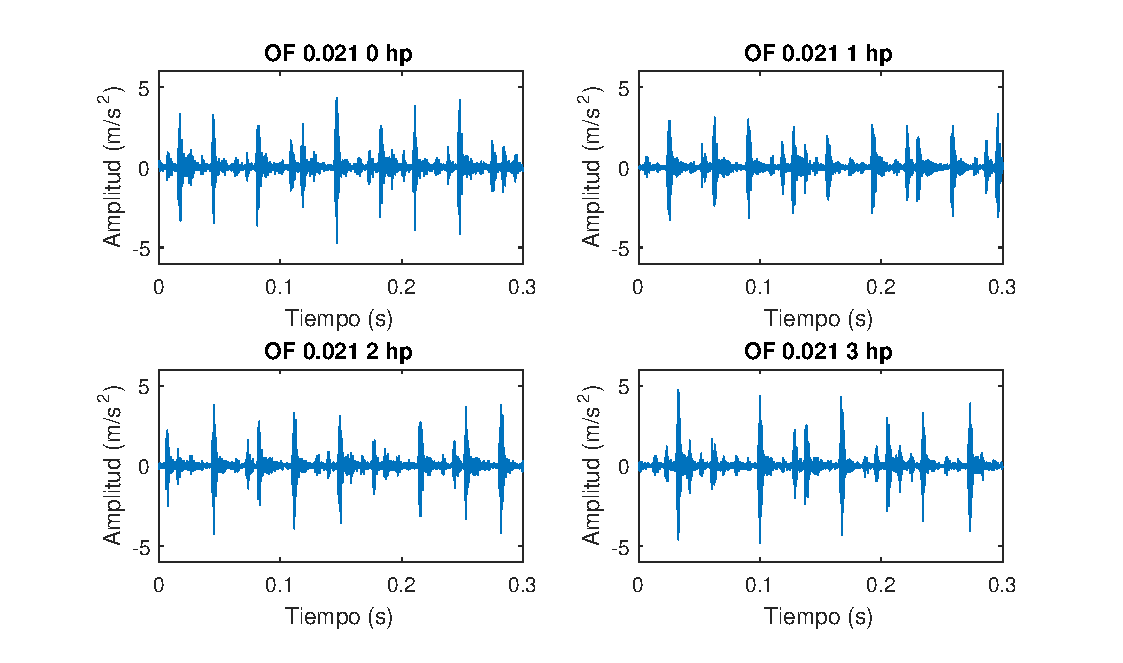
\includegraphics[scale=0.9]{./signalOF.eps}
  \caption{4 tipos de señal de vibración de un rodamiento, con una carga de 3 hp y 0,54 mm de diámetro de falla.}
  \label{fig:senales}
\end{figure}



\subsubsection{Reordenamiento, muestras de entrenamiento y testing}
\paragraph{}
Tal como lo indica el nombre de la subsección, este apartado explica el funcionamiento del re ordenamiento de las muestras de un \textit{dataset} y la división de las muestras en datos de entrenamiento y de \textit{testing}. Una vez que el proceso de extracción de características termina, el algoritmo codificado en MATLAB procede a reordenar las muestras y separarlas datos de \textit{training} y \textit{testing} con sus respectivas etiquetas. Los porcentajes que serán probados, y que afectan significativamente al modelo son los siguientes: 0.5, 0.6, 0.7 , 0.75 y 0.8.

\subsubsection{Ambiente de desarrollo}
\paragraph{}
La red neuronal profunda es construida con la \textit{toolkit} de MATLAB versión R2016a, y considera dos \textit{sparse} autoencoder apilados y una capa de neuronas con la función de transferencia softmax. La CPU utilizada para ejecutar estos algoritmos corresponde a un AMD(R) A10-5750M(TM) funcionando con el sistema operativo Windows 10(TM). 

\begin{figure}[ht]
  \centering
    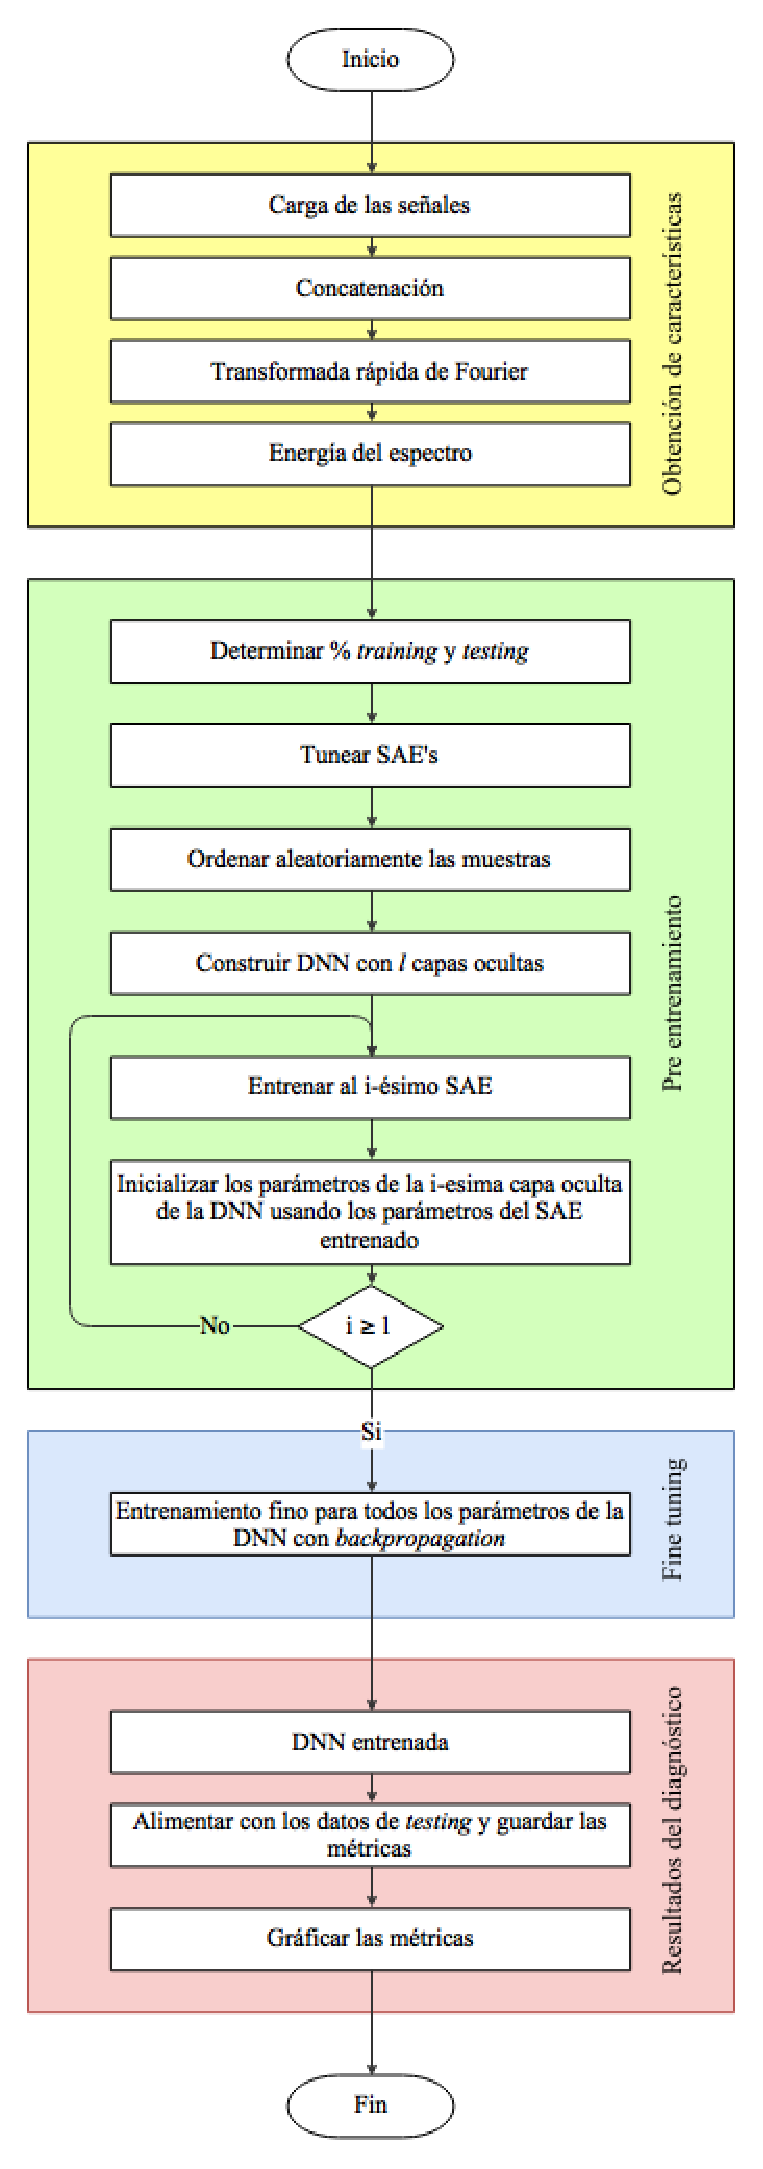
\includegraphics[scale=0.6]{./block.eps}
  \caption{Diagrama de flujo de los procesos que se llevan a cabo para entrenar y probar el modelo propuesto.}
  \label{fig:block}
\end{figure}

\subsection{Evaluando el desempeño}

\paragraph{}
Para evaluar el desempeño del modelo respecto a la calidad del diagnóstico se emplearan métricas que son habitualmente usadas en problemas de clasificación multiclase. Variadas investigaciones usan la validación cruzada para evaluar el aprendizaje del modelo, sin embargo, en este trabajo solo se efectuaran 30 ejecuciones por \textit{dataset} con el fin evaluar el rendimiento del modelo. A estas ejecuciones se les calculará la exactitud por ejecución, la exactitud (Ecc. \ref{acc}) promedio por clase, el F-score (Ecc. \ref{fscore}) o media armónica por clase y el F-score promedio por ejecución.

\paragraph{}
las Ecuaciones \ref{precision}, \ref{sensibilidad}, \ref{fscore} y \ref{acc} son calculadas con: verdaderos positivos (TP), verdaderos negativos (TN), falsos positivos (FP) y falsos negativos (FN) que plasman la calidad de la predicción realizada por el clasificador. La precisión (Ecc. \ref{precision}) representa el ratio o razón entre los correctamente identificados o verdaderos positivos y todos los positivos, mientras que la sensibilidad (Ecc. \ref{sensibilidad}) representa el ratio o razón entre los correctamente identificados y los negativos. El $F_{1}$score es la media armónica de los resultados de clasificación, y se usa este tipo de media en vez de la media aritmética porque es ideal cuando se trabaja con ratios o proporciones.

\begin{equation}
\label{precision}
Precisi\acute{o}n = \frac{TP}{TP+FP}
\end{equation}

\begin{equation}
\label{sensibilidad}
Sensibilidad = \frac{TP}{TP+FN}
\end{equation}

\begin{equation}
\label{fscore}
F_{1}score = \frac{2\cdot{Precisi\acute{o}n}\cdot{Sensibilidad}}{Precisi\acute{o}n\cdot{Sensibilidad}}
\end{equation}

\begin{equation}
\label{acc}
Exactitud = \frac{VP+VN}{VP+FP+VN+FN}
\end{equation} 

\subsection{Resultados}
\paragraph{}
Realizando las 30 ejecuciones para cada conjunto de datos, la red neuronal profunda se encargó de aprender complejas relaciones no lineales entre las características que le fueron entregadas. Logrando muy buenos resultados en especial para los dos \textit{datasets} más complicados (A y E) de acuerdo a las gráficas de exactitud y $F_{1}$score. En las pruebas fueron puestas apruebas distintas topologías, distintos tamaños de segmento, diferentes proporciones de entrenamiento y \textit{testing} y distintos valores para los hiperparámetros. Estos últimos corresponden a los términos que penalizan la función de costo de los \textit{sparse} autoencoder: $\lambda$ (weight decay), $\beta$ (spasity regularization) y $\rho$ (sparsity proportion).

\paragraph{}
Fue realmente complicado encontrar parámetros que mejoraran sustancialmente la exactitud en los \textit{datasets} de mayor interés. A pesar de esto, fue posible hallar un conjunto que diera buenos resultados, para el primer SAE: $\lambda=0.022$, $\beta=0.97$ y $\rho=0.02$ y para el segundo SAE $\lambda=0.0002$, $\beta=0.97$ y $\rho=0.25$. Respecto al tamaño de los segmentos, el mejor resultó en 2048 puntos por segmento tal como se comentaba en la descripción de los \textit{datasets}.

\paragraph{}
La cantidad óptima de unidades en la primera capa oculta resulto en 102 y para la segunda capa oculta 25, por lo que la red neuronal profunda llevó las características originales desde un espacio de alta dimensión a uno de menor dimensión, omitiendo las variaciones irrelevantes para la detección de patrones. La proporción ideal de muestras para entrenamiento y \textit{testing} fue de 70\% y 30\% respectivamente. Los resultados de las ejecuciones con estas configuraciones pueden ser observados en las gráficas que a continuación se discutirán.

\paragraph{}
Los resultados fueron muy buenos considerando la complejidad del problema
Los, el dataset A obtuvo en promedio para las 30 ejecuciones 99.8084\% de exactitud con una desviación estándar pequeña, por lo que el modelo entrega un buen diagnostico incluso en velocidad constante sin carga. Sorprendentemente en el dataset C la red neuronal profunda logra reconocer correctamente el estado de salud del rodamiento en cada una de las ejecuciones, superando a los resultados de diagnostico de \cite{jia} para ese dataset. 

\paragraph{}
El resultado que mayor satisfacción entrega, es el del dataset E, con un 99.9473 de exactitud promedio casi igualando a los resultados de una investigación a nivel de doctorado como lo es la de \cite{jia}. agregar explicacion

\paragraph{}
La Fig. \ref{fig:AccG} refleja el comportamiento de la exactitud a través de las ejecuciones revelando las ejecuciones donde baja considerablemente la exactitud y empeora el promedio de la prueba. la Fig. \ref{fig:Acc} detalla la exactitud promedio para las 10 clases, revelando las clases con mayores dificultades para el clasificador, como la clase 2, 3, 7 y 8 que corresponden a la bola y al anillo externo.

\begin{table}
\centering
\scalebox{0.9}{
\begin{tabular}[c]{c c c c c c}
\toprule
Dataset & Carga (hp) & Exactitud media global & Desviación estándar & Mínimo & Máximo\\
\midrule
A & 0 & 99.8084\% & $\pm$0.2756 & 99.4253\% & 100\%\\
\addlinespace
B & 1 & 99.9234\% & $\pm$0.2495 & 98.8506\% & 100\%\\
\addlinespace
C & 2 & 100\% & $\pm$0 & 100\% & 100\%\\
\addlinespace
D & 3 & 99.9425\% & $\pm$0.1754 & 99.4253\% & 100\%\\
\addlinespace
E & 0-3 & 99.9473\% & $\pm$0.1222 & 99.4253\% & 100\%\\
\bottomrule
\end{tabular}}
\caption{Resultados del testing para cada dataset.}
\label{table:results}
\end{table}

\begin{figure}[ht]
  \centering
    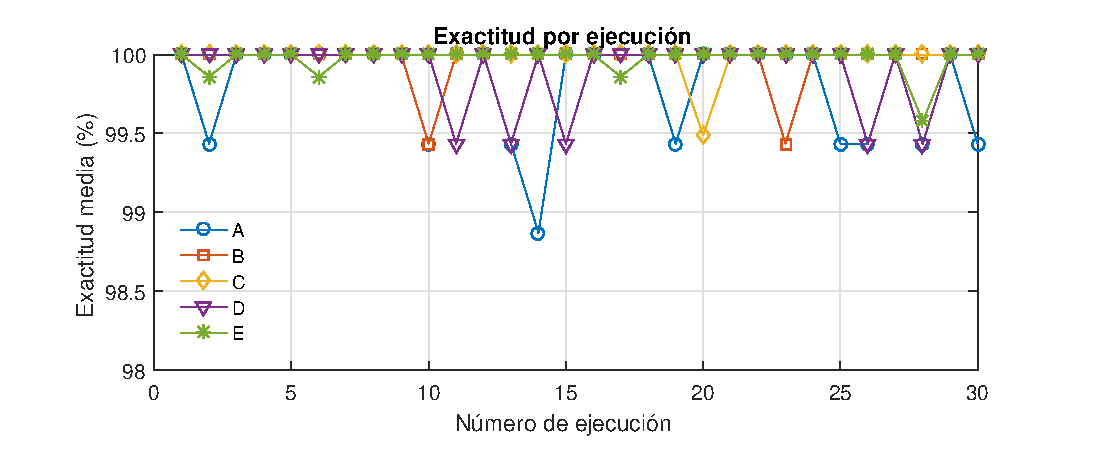
\includegraphics[scale=0.5]{./AccG.eps}
  \caption{Diagrama con la exactitud del clasificador en 30 ejecuciones.}
  \label{fig:AccG}
\end{figure}

\begin{figure}[ht]
  \centering
    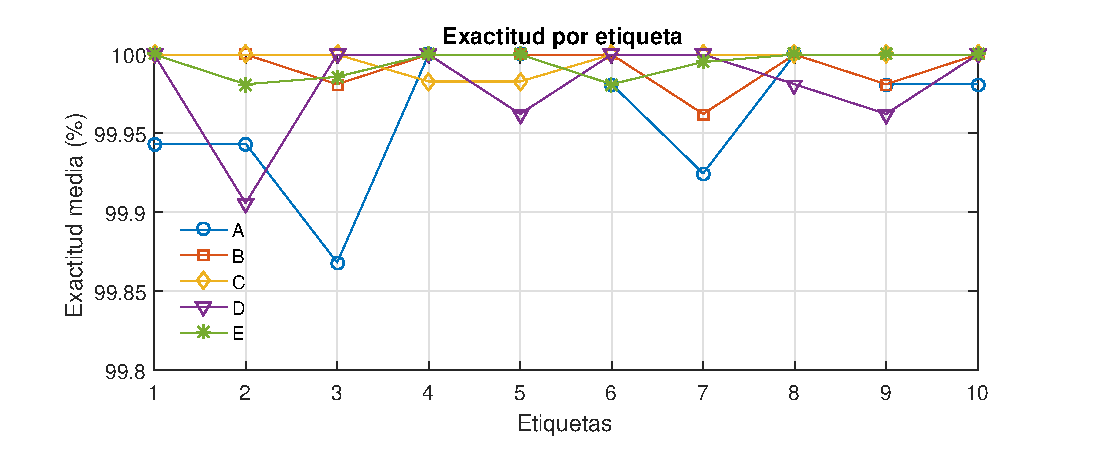
\includegraphics[scale=0.5]{./Acc.eps}
  \caption{Diagrama con la exactitud promedio de las 30 ejecuciones para cada una de las 10 clases.}
  \label{fig:Acc}
\end{figure}

\begin{figure}[ht]
  \centering
    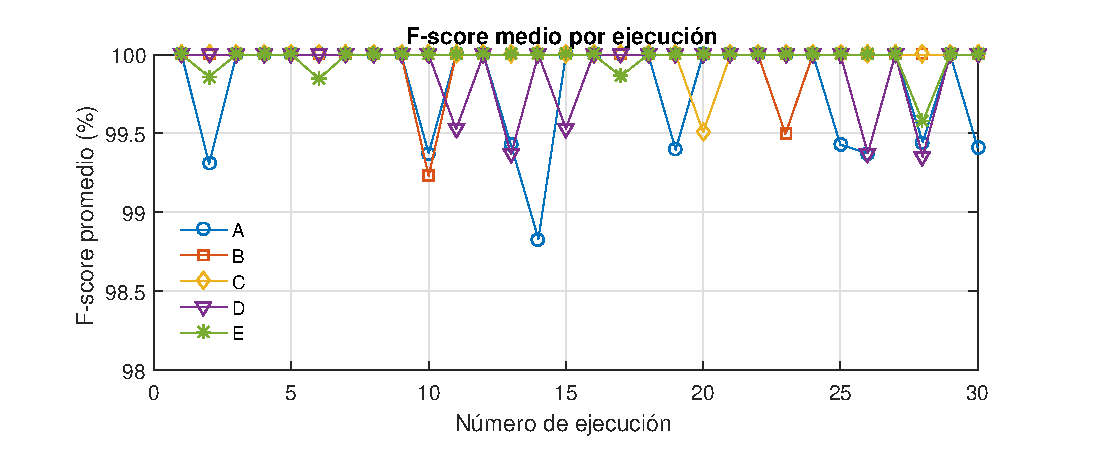
\includegraphics[scale=0.5]{./FscG.eps}
  \caption{Diagrama con el $F_{1}$score de cada una de las 30 ejecuciones.}
  \label{fig:FscG}
\end{figure}

\begin{figure}[ht]
  \centering
    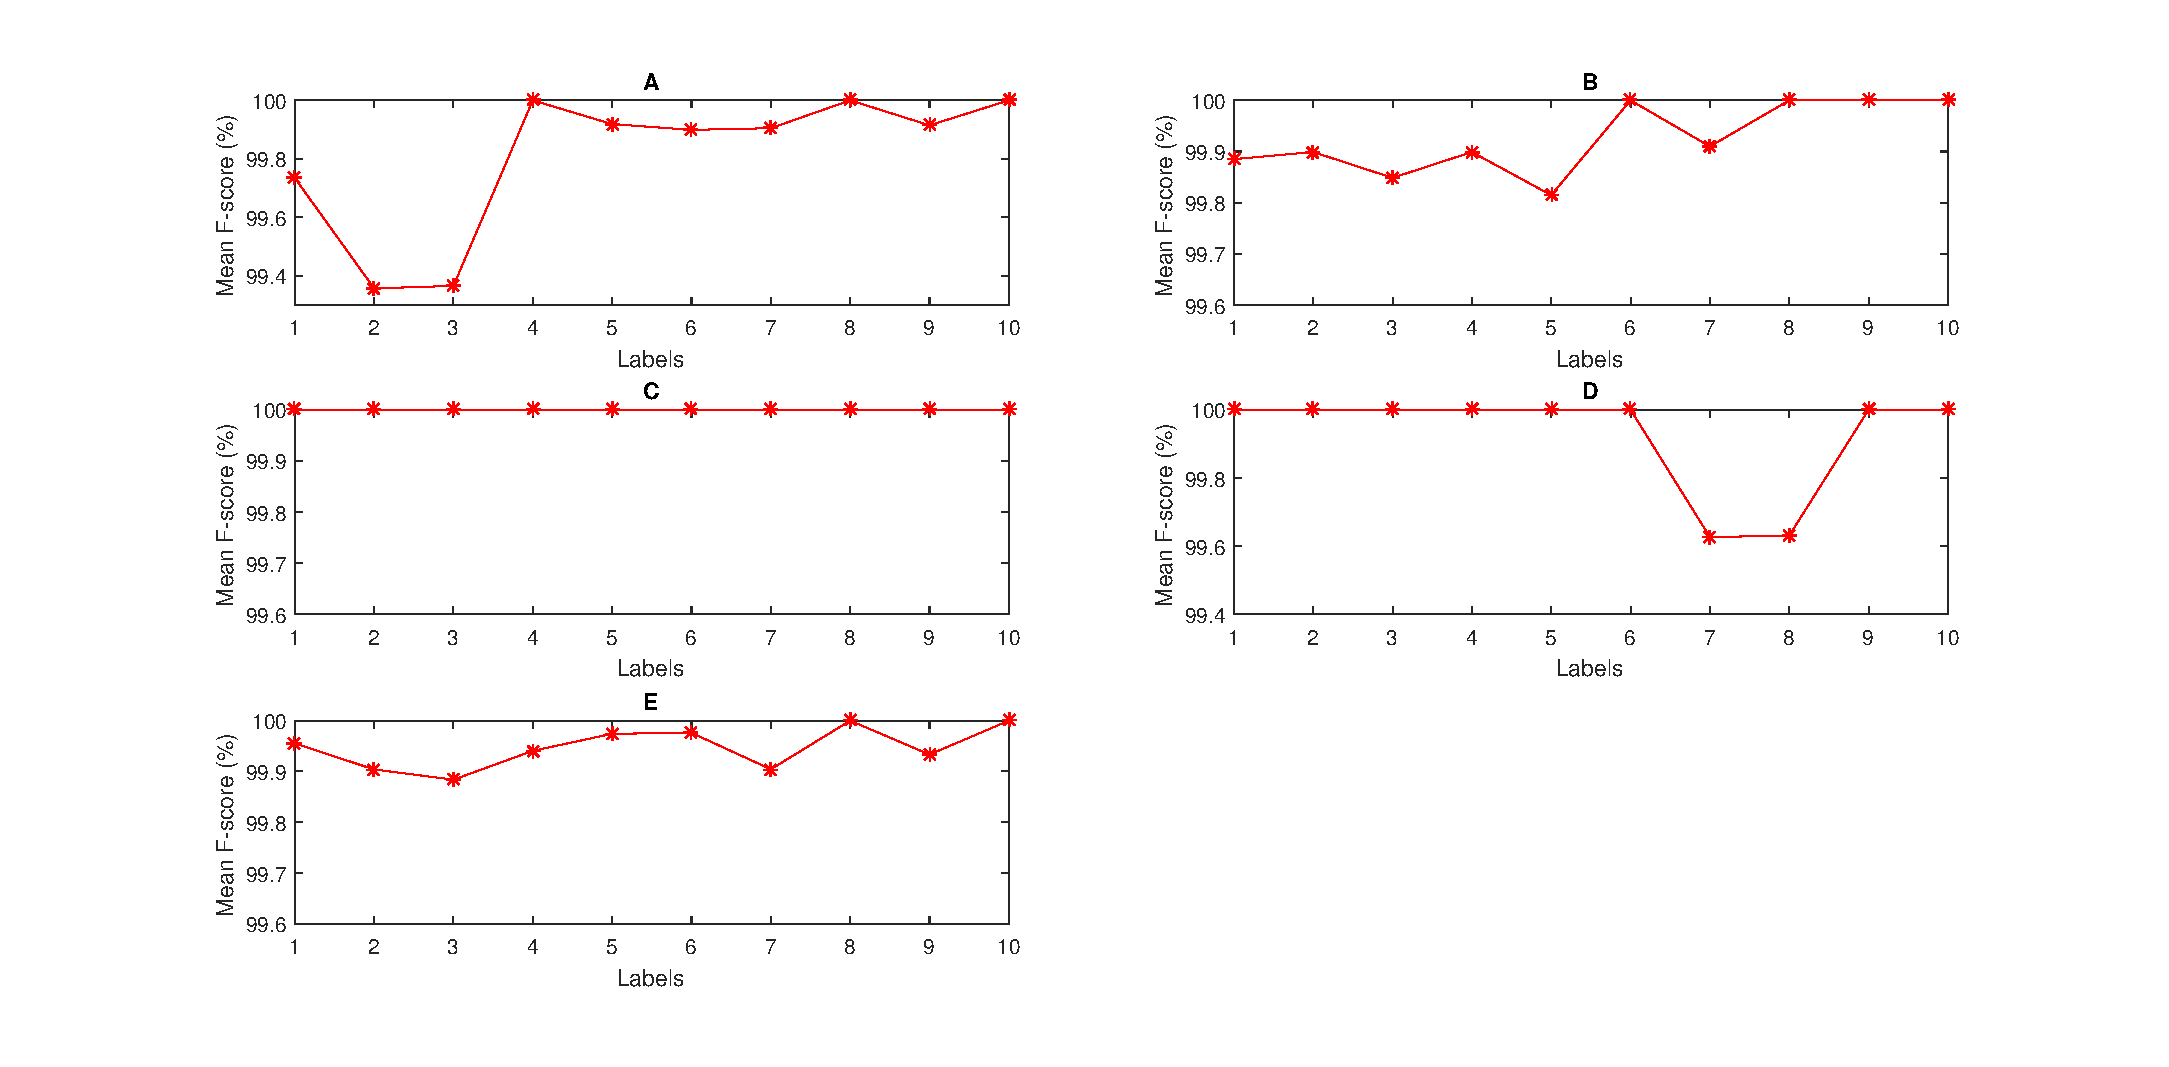
\includegraphics[scale=0.5]{./Fsc.eps}
  \caption{Diagrama con el $F_{1}$score promedio de las 30 ejecuciones para cada una de las 10 clases.}
  \label{fig:Fsc}
\end{figure}

\subsection{Conclusión}
\paragraph{}
Como conclusión, la red neuronal profunda compuesta por \textit{sparse} autoencoders apilados puede lograr un desempeño asombroso respecto a la exactitud del diagnostico (a nivel de doctorado), siempre que encuentre una buena configuración de hiperparámetros, los porcentajes de entrenamiento y de \textit{testing} y una buena topología de las capas ocultas. Es por esto que las redes neuronales profundas, muy utilizadas en reconocimiento de imágenes, están ganando territorio en otras áreas de investigación, como lo es el diagnostico de fallas en rodamientos mediante su señal de vibración. Sin embargo, este modelo de monitoreo de condiciones tiene la desventaja de un excesivo tiempo de \textit{tuning} de los hiperparámetros, si bien la técnica de extracción de características es rápida computacionalmente; el proceso de encontrar parámetros para los \textit{sparse} autoencoders es lento y engorroso. Por lo que puede resultar poco alentador calibrar el modelo por el tiempo que demanda encontrar las variables que potencian al clasificador. De esta misma manera, los tiempos de ejecución tampoco son los mejores, el algoritmo del gradiente conjugado necesita bastantes iteraciones (menos que el descenso del gradiente) para acercarse al optimo global de la función de costos. Entonces, las redes neuronales profundas son una excelente herramienta de diagnostico de fallas para este problema muy complejo, pero requiere un sacrificio no menor a la hora de buscar parámetros para los SAE.

\clearpage

\begin{thebibliography}{9}
\bibitem{seeraa} Manjeevan Seeraa, M.L. Dennis Wonga \& Asoke K. Nandic (2017). Classification of ball bearing faults using a hybrid intelligent model. \textit{Applied Soft Computing}, \textit{57}, 427–435.

\bibitem{zhan} Yimin Zhan \& Chris K. Mechefske (2007). Robust detection of gearbox deterioration using compromised
autoregressive modeling and Kolmogorov–Smirnov test statistic—Part I: Compromised autoregressive modeling with the
aid of hypothesis tests and simulation analysis. \textit{Mechanical Systems and Signal Processing}, \textit{21}, 1953–1982.

\bibitem{issam} Issam Attoui, Nadir Fergani, Nadir Boutasseta, Brahim Oudjani \& Adel Deliou (2017). A new time–frequency method for identification and classification of ball bearing faults. \textit{Journal of Sound and Vibration}, \textit{397}, 241-265.

\bibitem{fu} Yunxiao Fu, Limin Jia, Yong Qin \& Jie Yang (2016). Product Function Correntropy and Its Application in Rolling bearing Fault Identification. \textit{Measurement}, 88-99.

\bibitem{li} Wei Li, Zhencai Zhu, Fan Jiang, Gongbo Zhou \& Guoan Chen (2015). Fault diagnosis of rotating machinery with a novel statistical feature extraction and evaluation method. \textit{Mechanical Systems and Signal Processing}, \textit{50-51}, 414-426.

\bibitem{guo} Hong Guo, Lindsay B. Jack \& Asoke K. Nandi (2005). Feature Generation Using Genetic Programming With Application to Fault Classification. \textit{IEEE Transactions on Systems, Man, and Cybernetics, Part B (Cybernetics)}, \textit{35}(1), 89-99.

\bibitem{zhu} Xiaoran Zhu, Youyun Zhang \& Yongsheng Zhu (2012). Intelligent fault diagnosis of rolling bearing based on kernel neighborhood rough sets and statistical features. \textit{Journal of Mechanical Science and Technology}, \textit{26}(9), 2649-2657.

\bibitem{jia} Feng Jia, YaguoLei, Jing Lin, Xin Zhou \& Na Lu (2015). Deep neural networks: A promising tool for fault characteristic mining and intelligent diagnosis of rotating machinery with massive data. \textit{Mechanical Systems and Signal Processing}, \textit{72-73}, 303-315.

\bibitem{yu} Yang Yu, YuDejie \& Cheng Junsheng (2006). A roller bearing fault diagnosis method based
on EMD energy entropy and ANN. \textit{Journal of Sound and Vibration}, \textit{294}, 269–277. 

\bibitem{chang} Changting Wang \& Robert X. Gao (2002). Wavelet Transform with Spectral Post-Processing for
Enhanced Feature Extraction. \textit{IEEE Instrumentation and Measurement Technology Conference}, \textit{52}(4), 1296-1301.

\bibitem{ran} Ran Zhang, Zhen Peng, Lifeng Wu, Beibei Yao \& Yong Guan (2017). Fault Diagnosis from Raw Sensor Data Using Deep Neural Networks Considering Temporal Coherence. \textit{Sensors}, \textit{17}(3), 549-566.

\bibitem{ali} Jaouher Ben Ali, Nader Fnaiech, Lotfi Saidi, Brigitte Chebel-Morello \& Farhat Fnaiech (2015). Application of empirical mode decomposition and artificial neural network for automatic bearing fault diagnosis based on vibration signals. \textit{Applied Acoustics}, \textit{89}, 16–27.

\bibitem{wu} Lifeng Wu, Beibei Yao, Zhen Peng \& Yong Guan (2017). Fault Diagnosis of Roller Bearings Based on a Wavelet Neural Network and Manifold Learning. \textit{Applied Science}, \textit{7}, 158-168. 

\bibitem{rai} V.K. Rai \& A.R. Mohanty (2007). Bearing fault diagnosis using FFT of intrinsic mode functions in Hilbert–Huang transform. \textit{Mechanical Systems and Signal Processing}, \textit{21}, 2607–2615.

\bibitem{anthony} Wheeler, Anthony J. \& Ganji, Ahmad R. (2009). \textit{Introduction to Engineering Experimentation} (3rd ed., pp. 107-117). New Jersey: Prentice Hall.

\bibitem{robert} Gray, Robert M. \& Goodman, Joseph W. (1995). \textit{Fourier Transforms: An Introduction for Engineers} (1st ed., pp. 53-57). New York: Springer.

\bibitem{shao} Shao Haidong, Jiang Hongkai, Zhao Huiwei \& Wang Fuan (2017). A novel deep autoencoder feature learning method for rotating machinery fault diagnosis. \textit{Mechanical Systems and Signal Processing}, \textit{95}, 187-204. 

\bibitem{song} Song-Zhi Su, Zhi-Hui Liu, Su-Ping Xu, Shao-Zi Li \& Rongrong Ji (2014). Sparse auto-encoder based feature learning for humanbody detection in depth image. \textit{Signal Processing}, \textit{112}, 43-52.

\bibitem{yufeng} Yufeng Zhang, Zhenyu Guo, Weilian Wang, Side He, Ting Lee \& Murray Loew (2003). A comparison of the wavelet and short-time fourier transforms for Doppler spectral analysis. \textit{Medical Engineering \& Physics}, \textit{25}, 547-557.

\bibitem{aure} Aurelien Prudhom, Jose Antonino-Daviu, Hubert Razik \& Vicente Climente-Alarcon (2015). Time-frequency vibration analysis for the detection of motor damages caused by bearing currents. \textit{Mechanical Systems and Signal Processing}, \textit{84}, 747-762.

\bibitem{chen} Zhiqiang Chen, Shengcai Deng, Xudong Chen, Chuan Li, René-Vinicio Sanchez \& Huafeng Qin (2017). Deep neural networks-based rolling bearing fault diagnosis. \textit{Microelectronics Reliability}, \textit{75}, 327-333.

\bibitem{konar} P. Konar \& P. Chattopadhyay (2011). Bearing fault detection of induction motor using wavelet and Support Vector Machines (SVMs). \textit{Applied Soft Computing}, \textit{11}, 4203-4211.

\bibitem{mao} Wentao Mao, Jianliang He, Yuan Li \& Yunju Yan (2017). Bearing fault diagnosis with auto-encoder extreme learning machine: A comparative study. \textit{Proceedings of the Institution of Mechanical Engineers, Part C: Journal of Mechanical Engineering Science}, \textit{231}(8), 1560-1578.

\bibitem{kanpaj} Kanpaj Gupta \& M.K. Pradhan (2017). Fault detection analysis in rolling element bearing: A review, \textit{Materials Today: Proceedings}, \textit{4}, 2085-2094.

\bibitem{mining} Witten, Ian H. \& Frank, Eibe \& Hall, Mark A. \& Pal, Christopher J. (2016). \textit{Data Mining: Practical Machine Learning Tools and Techniques-Morgan Kaufmann} (4th ed., pp. ), Morgan Kaufmann.

\bibitem{haykin} Haykin, Simon. (2009). \textit{Neural Networks and Learning Machines} (3rd ed., pp.), Pearson.

\bibitem{ranzato} Marc’Aurelio Ranzato, Y-Lan Boureau \& Yann LeCun (2008). Sparse feature learning for deep belief networks. Adv.NeuralInf.Process.Sys. 1185–1192.

\bibitem {du}Erzhu Li, Peijun Du, Alim Samat, Member, Yaping Meng y Meiqin Che, \textit{Mid-Level Feature Representation via Sparse Autoencoder for Remotely Sensed Scene Classification}, IEEE J. Sel. Top. Appl. Earth Obs. Remote Sens. 10 1068–1081, 2017

\bibitem {case}Case Western Reserve University Bearing Data Center, \textit{Bearing vibration data set}, http://csegroups.case.edu/bearingdatacenter/pages/12k-drive-end-bearing-fault-data, (visitado el 30-08-2017).

\bibitem {allen}Jont B. Allen y Lawrence R. Rabiner, \textit{A Unified Approach to Short-Time Fourier Analysis
and Synthesis}, Proceedings Of The IEEE, VOL. 65, NO. 11, 1977


\end{thebibliography}

\end{document}
